\section{Usability and Community} \label{section:usability}
\large \textbf{Apache Kafka}\\
\normalsize
\textbf{Active community}\\
The community of Kafka is very active. Since it is created in 2012, the GitHub repository of Kafka has been regularly committed. Starting from the end of 2015, the activity of the community increases significantly with an average of roughly 20 commits per day. In the top 30 contributors, each of them has made more than 50 commits to the project. Many of the contributors are from Confluent which is the company founded by the creators of Kafka. Nevertheless, there are also numerous contributors coming from different organizations and institutions as well.

\begin{figure}[h]
	\centering
	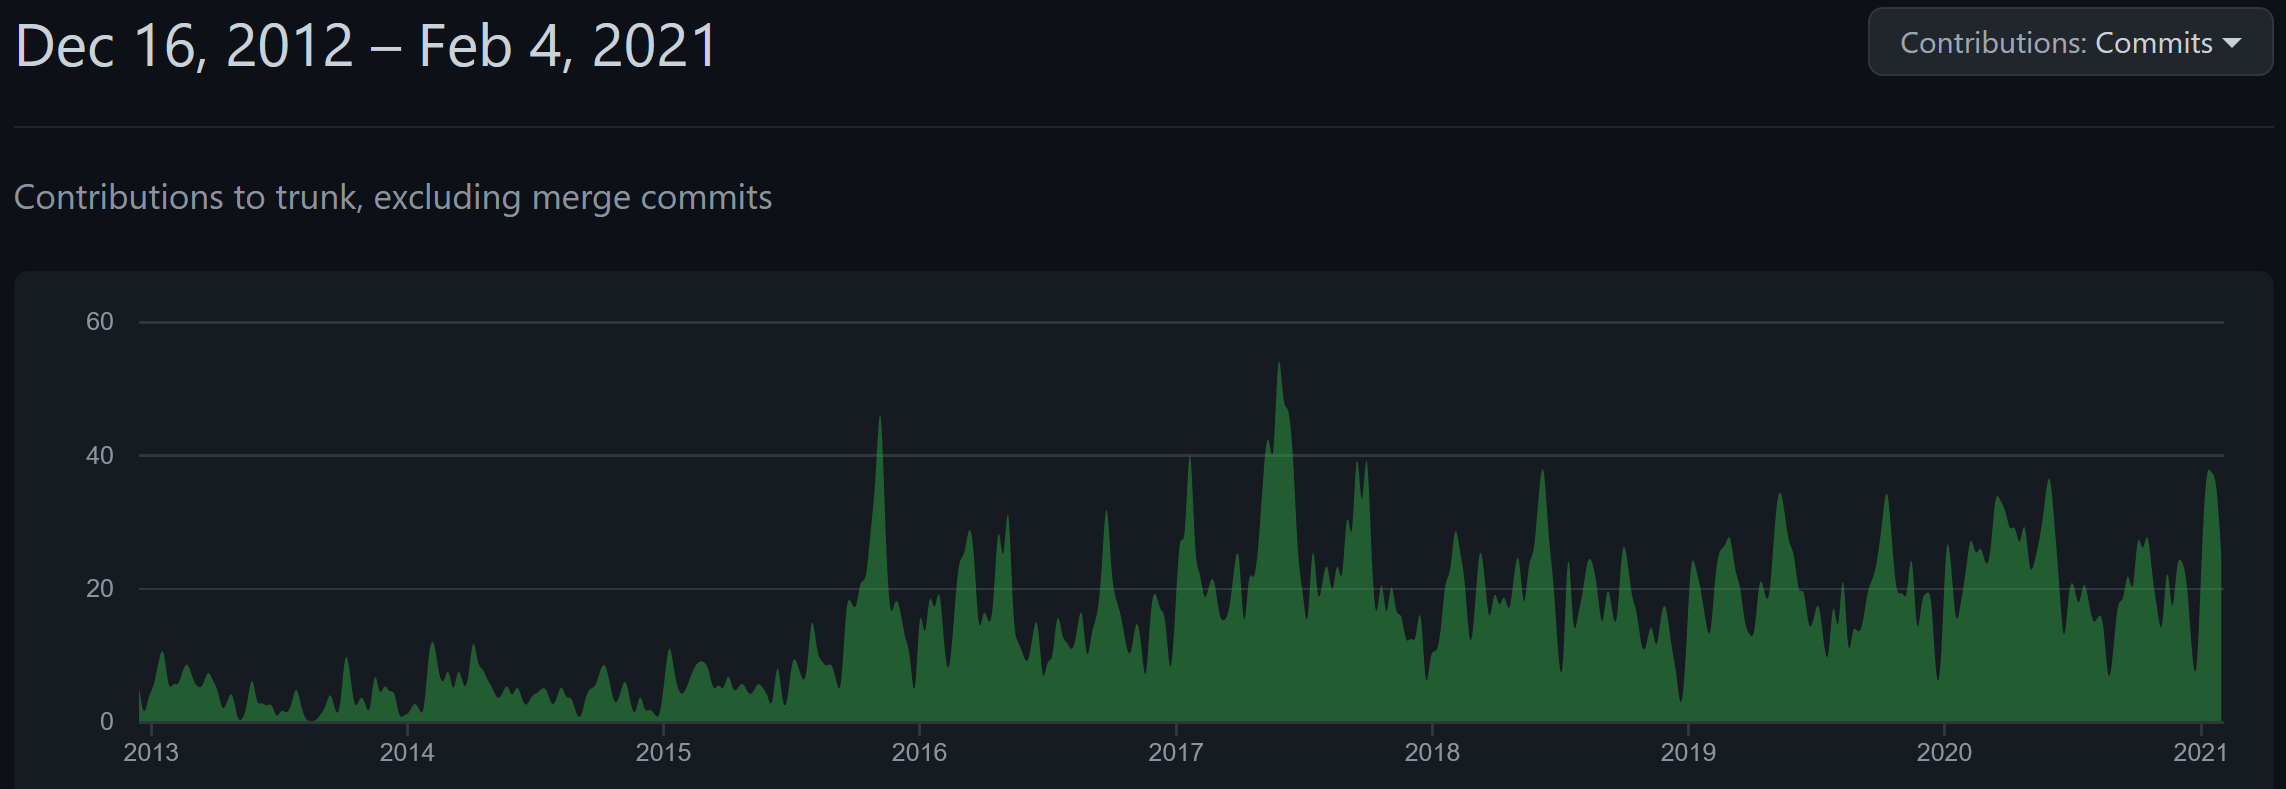
\includegraphics[width=11cm,height=4.5cm]{images/community-kafka.png}
	\caption{Contributions to Kafka on GitHub \cite{kafkarepo}.}
	\label{fig:communitykafka}
\end{figure}

In December 2020, more than 50 contributors made 160 commits to the repository. In this month, there are also around 50 new pull requests and more than 100 merged pull requests on the project.

\large \textbf{Apache Pulsar}\\
\normalsize
\textbf{Active community}\\
\begin{figure}[h]
	\centering
	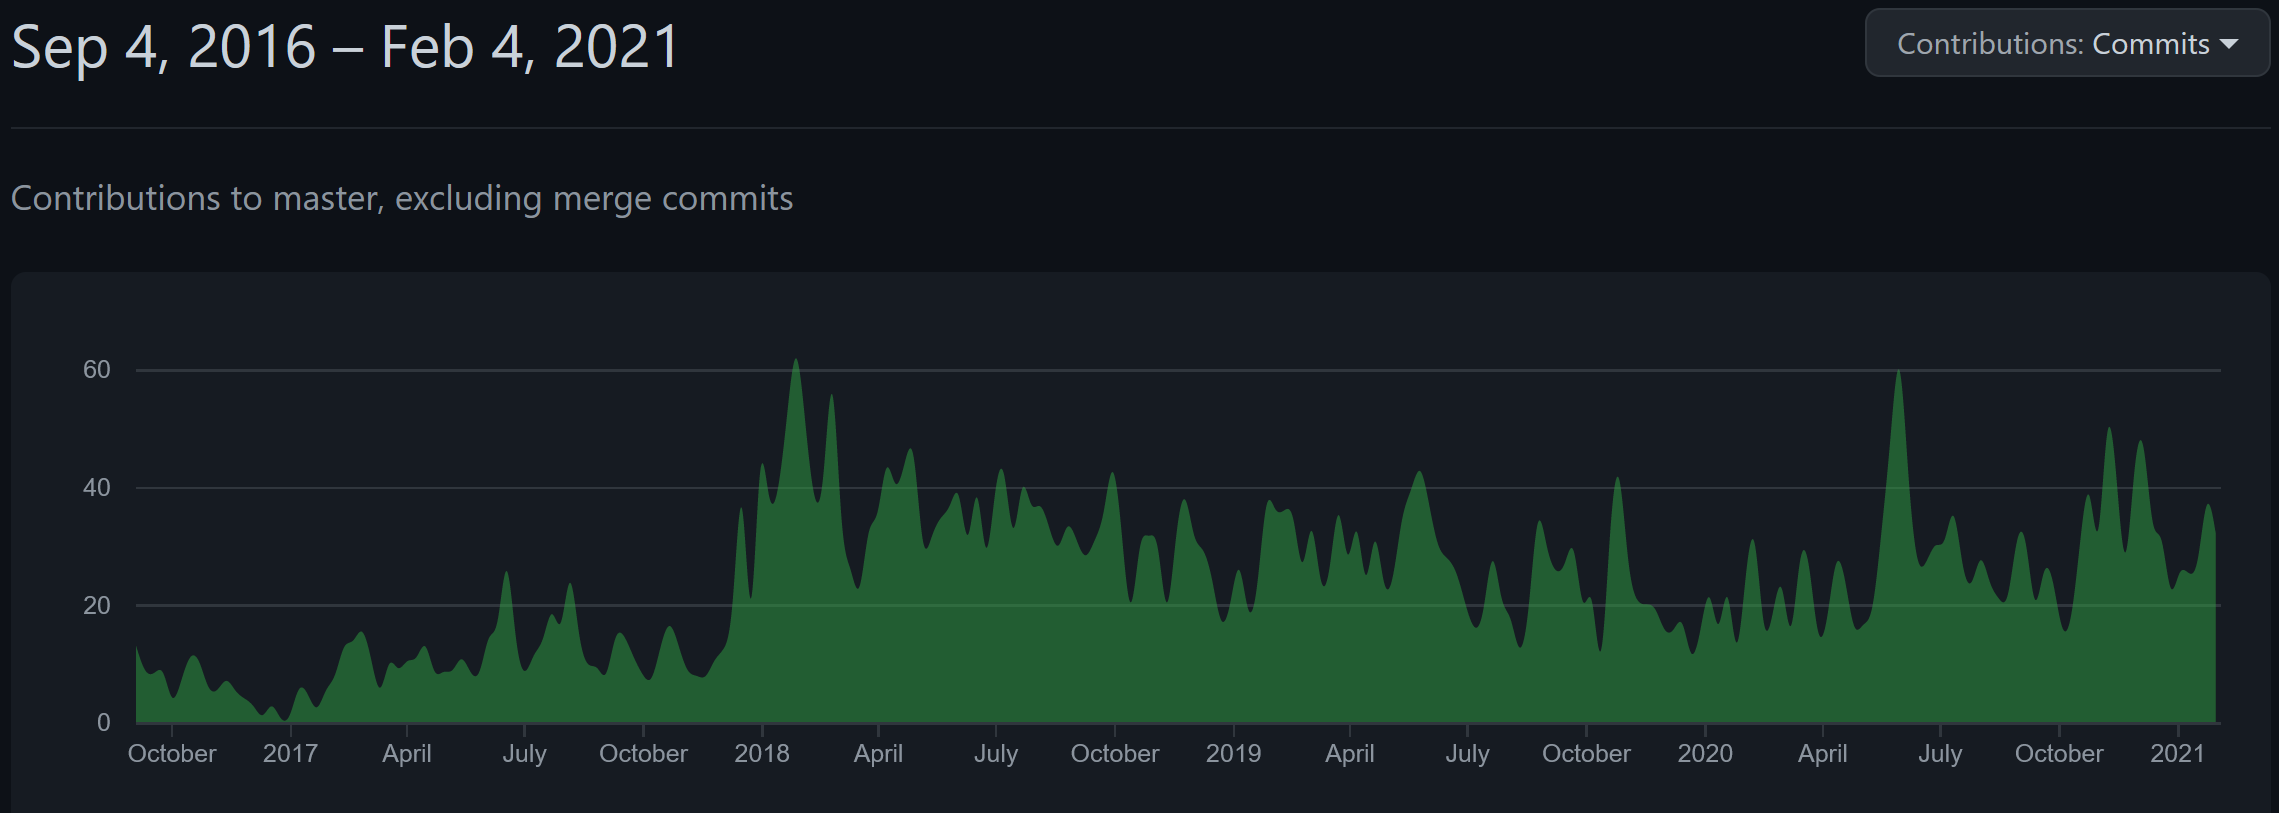
\includegraphics[width=11cm,height=4.5cm]{images/community-pulsar.png}
	\caption{Contributions to Pulsar on GitHub \cite{pulsarrepo}.}
	\label{fig:communitypulsar}
\end{figure}

Since 2016, the Apache Pulsar has been steadily contributed by the community. From 2018, Apache Pulsar has gained more interest from the community with the increase in commits to about 30 commits per day. Each of the top 20 contributors have made more than 50 commits to the project. Many top contributors come from Splunk and Streamnative which are two companies providing managed services based on Apache Pulsar. In addition, there are also many contributors from the different organization actively engaging in the project.

In December 2020, 360 commits have been made by 56 contributors on the Pulsar project. Moreover, more than 200 pull requests are active during this time. 

\large \textbf{NATS Streaming}\\
\normalsize
\textbf{Active community}\\
From the data on GitHub, the NATS Streaming project is not very active, especially since 2018 with an average of around 3 to 4 commits per day. Moreover, only the top 3 contributors have made most of the commits to the project and two of them are from Synadia which is the company creating the NATS system. The other contributors only make minors commit to the project. 

\begin{figure}[h]
	\centering
	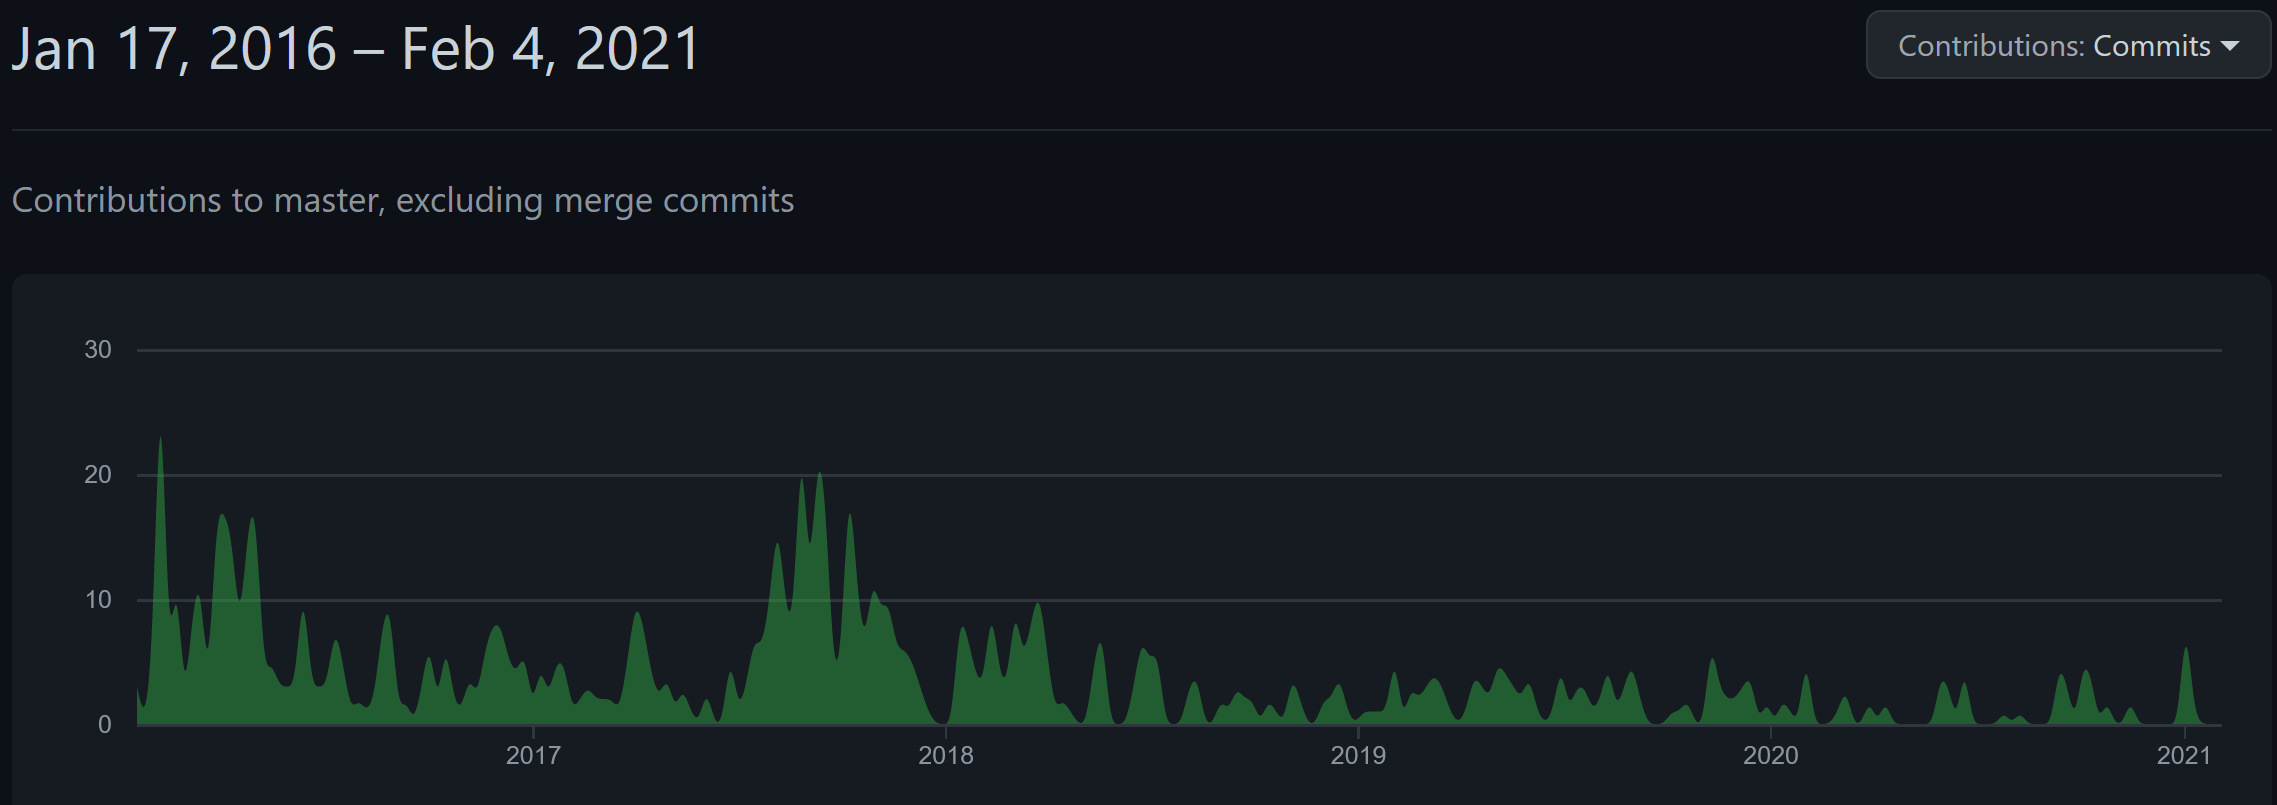
\includegraphics[width=11cm,height=4.5cm]{images/community-nats.png}
	\caption{Contributions to NATS Streaming on GitHub \cite{natsrepo}.}
	\label{fig:communitynats}
\end{figure}

In the month December 2020, no commit has been made on the NATS Streaming repository. In addition, during this month, no pull request is created or merged. 

